\documentclass[letterpaper,11pt]{article}

%-----------------------------------------------------------
\usepackage[empty]{fullpage}
\usepackage{hyperref}
\usepackage{textcomp}
\usepackage{xcolor}
\usepackage{graphicx}
\usepackage{wrapfig}
\usepackage{float}
\raggedbottom
\raggedright
\setlength{\tabcolsep}{0in}
\graphicspath { {.} }

\ifdefined\darkmode
	\definecolor{title_bg}{RGB}{66, 66, 70}
	\definecolor{link_fg}{RGB}{38, 152, 186}
	\definecolor{bg}{RGB}{0, 0, 0}
	\definecolor{fg}{RGB}{255, 255, 255}
\else
	\definecolor{title_bg}{gray}{0.80}
	\definecolor{link_fg}{RGB}{26, 13, 171}
	\definecolor{bg}{RGB}{255, 255, 255}
	\definecolor{fg}{RGB}{0, 0, 0}
\fi

\pagecolor{bg}

% Adjust margins to 0.5in on all sides
\addtolength{\oddsidemargin}{-0.5in}
\addtolength{\evensidemargin}{-0.5in}
\addtolength{\textwidth}{1.0in}
\addtolength{\topmargin}{-0.5in}
\addtolength{\textheight}{1.0in}

%-----------------------------------------------------------
%Custom commands
\newcommand{\resitem}[1]{\item #1 \vspace{-2pt}}
	\newcommand{\resheading}[1]{{\vspace{.2in} \large \colorbox{title_bg}{\begin{minipage}{\textwidth}{\textbf{#1 \vphantom{p\^{E}}}}\end{minipage}}}}

\newcommand{\ressubheading}[4]{
\begin{tabular*}{7.1in}{l@{\extracolsep{\fill}}r}
		\textbf{#1} & #2 \\
		\textit{#3} & \textit{#4} \\
\end{tabular*}\vspace{0pt}}
%-----------------------------------------------------------

\color{fg}
\begin{document}

\begin{minipage}{.70\linewidth}
	\begin{center}
		\textbf{\Large Vasyl Horbachenko} \\
		Frankfurt am Main, Germany \\
		vasyl.horbachenko@gmail.com \\
		\href{https://shdwp.github.io/about/}{\textcolor{link_fg}{\underline{https://shdwp.github.io/about/}}} \\

		\vspace{0.2in}
		\resheading{Skills}
		\begin{description}
			\item[Code:]
				C\#, C++, C, HLSL, MSIL
			\item[Platforms:]
				Desktop (Unity, OpenGL), Mobile (iOS, cross-platform),\\ VR (OpenXR, Meta Quest)
			\item[Communication:]
				English (Proficient), German (Intermediate), \\Ukrainian (Native), Russian (Proficient)
		\end{description}
	\end{center}
\end{minipage}
\hfill
\begin{minipage}{.26\linewidth}
	\begin{flushright}
		\fbox{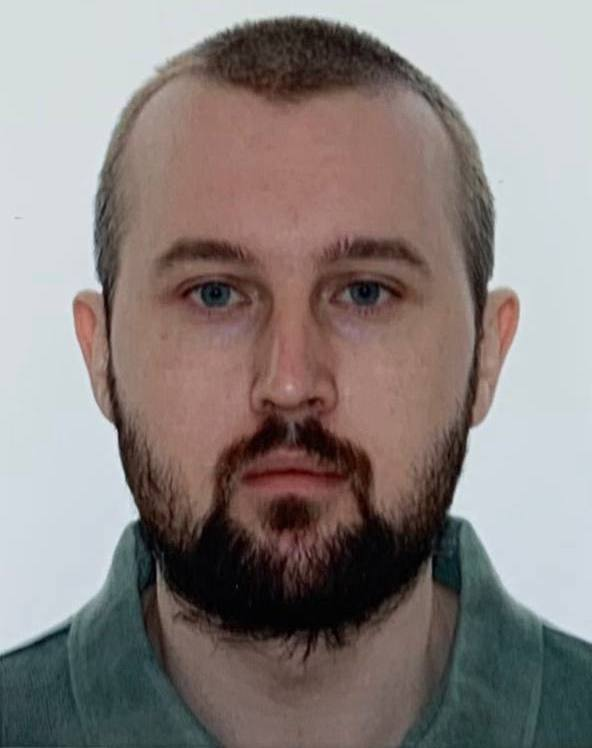
\includegraphics[scale=0.25]{pic2}}
	\end{flushright}
\end{minipage}
\begin{description}
	\item[Applications:]
		Unity Editor, Blender, git, IntelliJ, Jira, Gitlab, doxygen
	\item[Miscellaneous:]
		Git Flow, CI/CD, testing (unit, UI, integration), UML
\end{description}

\resheading{Education}
\begin{itemize}
\item
	\ressubheading{Chernigiv State Technological University}{Chernigiv, Ukraine}{Computer Science, Bachelor}{Sep. 2012 - May. 2017}
\end{itemize}

\resheading{Relevant Work Experience}
\begin{itemize}
	\item
		\ressubheading{Thoughtfish}{Remote, Berlin}{Unity Developer}{July 2023 - Present}

		Working as a Senior Unity engineer on PC \& VR projects. Mostly dealing with architecture, rendering and performance.
		\begin{itemize}
				\resitem{Tech leading a team of coders - code organization / MR reviews / architecture}
				\resitem{CI/CD setup, technical documentation, Unity Package code-sharing workflows}
				\resitem{VR project dealing a lot with optimization - both memory and frametimes}
				\resitem{Voxel meshing with LODs, rendering millions of differently shaped blocks}
		\end{itemize}

	\item
		\ressubheading{gamigo}{Remote, Berlin}{Unity Developer}{August 2022 - July 2023}

		Working with a team or developers, designers and artists to create a mobile game.
		\begin{itemize}
				\resitem{Software system design and planning}
				\resitem{Gameplay programming}
				\resitem{SRP graphics programming}
		\end{itemize}

	\item
		\ressubheading{Build1}{Remote, Kyiv}{Unity Developer}{December 2020 - August 2022}

		Working with a team of game designers \& programmers on various projects.
		\begin{itemize}
				\resitem{Multiplayer code development}
				\resitem{Custom shading \& rendering pipelines}
				\resitem{Experience with \textbf{il2cpp} and \textbf{webgl}}
				\resitem{Lots of optimization work due low-end devices targeted}
				\resitem{Contributions to in-house MVC framework}
		\end{itemize}

	\item
		\ressubheading{Self-employed}{Lviv}{General Game Developer}{December 2019 - December 2020}

		Implementing ideas and working on learning projects revolving around game development and 3D graphics (see \href{https://shdwp.github.io/about/projects/}{\textcolor{link_fg}{\underline{projects page}}}). \\
		\begin{itemize}
				\resitem{Development using Unity Engine}
				\resitem{Reverse-engineering Unity games}
				\resitem{OpenGL and C++ game engine development, scripting language integration (Lua)}
		\end{itemize}

	\item
		\ressubheading{Globallogic}{Lviv}{Flutter developer}{Aug 2019 - December 2019}
		
		Working on a number of ``proof-of-concepts'' with \textbf{Dart}/\textbf{Flutter}, mainly revolving around Bluetooth and native plugin communication.
		\begin{itemize}
				\resitem{Adopting existing BLE communication code as a Flutter plugin, designing communication layer between native and cross-platform}
				\resitem{Making a flutter application that uses forementioned plugin to communicate with Bluetooth device}
		\end{itemize}

	\item
		\ressubheading{Globallogic}{Lviv}{iOS Developer}{Jul 2017 - Aug 2019}

		Developer and team lead for a large healthcare-related Bluetooth application.
		\begin{itemize}
				\resitem{Coordination between 4 teams in different locations; the application was a \textit{``connecting piece''} bringing everything together}
				\resitem{Full blown QA: automated tests, unit tests, integration tests \& manual runs}
				\resitem{Mobile team consisted of 10+ people (around 50-70 in total for the whole project)}
		\end{itemize}

		My responsibilities on the project:
		\begin{itemize}
				\resitem{Core \textbf{BLE} interactions runtime architecture \& implementation}
				\resitem{Firmware-over-the-air implementation, sending binary images over BLE using custom TCP-like protocol}
				\resitem{Bluetooth communication debugging using \textbf{Frontline BLE sniffer}}
				\resitem{Separating the application codebase into an \textbf{SDK} for a family of medical devices}
				\resitem{Team Leading and team coordination at the later stages}
		\end{itemize}

\end{itemize}

\resheading{Awards}
\begin{itemize}
	\item
		\ressubheading{Junior Academy of Sciences of Ukraine Scholarship}{Kyiv, JASU}{Computer Science}{2010-2012}

		Scholarship from \href{http://man.gov.ua/en}{\textcolor{link_fg}{\underline{JASU}}}, a Junior section of Ukrainian Academy of Sciences (during high school); works related to IT integration into the education process.
	\item
		\ressubheading{Product copyright registration certificate}{Kyiv, JASU}{Certificate \textnumero40491}{2014}

		Was also awarded a copyright registration certificate as a result of my involvement in JASU.
\end{itemize}

\iffalse
\resheading{Other Notable Projects}
\begin{itemize}
	\item
		\ressubheading{OsaVR}{Opensource}{Creator}{August 2020 - Present}

		\href{https://github.com/shdwp/osavr}{\textcolor{link_fg}{\underline{Open-source Unity application}}} to simulate \textit{9K33M Osa SAM System} with target of making a VR game out of it.
		\begin{itemize}
				\resitem{Unity HDRP project with custom assets}
				\resitem{X-Band Radar real time simulation with radar cross-section approximation based on target mesh, all running on GPU as a custom renderer pass}
				\resitem{Lower-level plugins written in C for GPU rendered radar images processing, running in separate threads}
				\resitem{Custom shaders for instruments made with both Shader Graph and HLSL}
		\end{itemize}

	\item
		\ressubheading{openrunner}{Opensource}{Creator}{June 2020 - Present}
		
		\href{https://github.com/shdwp/openrunner}{\textcolor{link_fg}{\underline{openrunner}}} is a open-source OpenGL implementation of collectible card game \textit{Android: Netrunner}.
		\begin{itemize}
				\resitem{Game engine written in C++, with Lua API for the game logic implementation}
				\resitem{Fully cross platform source code}
		\end{itemize}

	\item
		\ressubheading{UIExtenderLib for M\&B Bannerlord II}{Opensource}{Creator, maintainer}{April 2020 - Present}

		\href{https://github.com/shdwp/UIExtenderLib}{\textcolor{link_fg}{\underline{Library}}} for modification developers to solve problems of multiple mods altering same game files.
		\begin{itemize}
				\resitem{Application code reverse-engineering}
				\resitem{MSIL patches made to be resursively added by each user of the library}
				\resitem{Runtime assembly builder to be used with Harmony}
		\end{itemize}

	\item
		\ressubheading{Dynamic campaign engine for Digital Combat Simulator}{Opensource}{Creator, maintainer}{May 2018 - Present}

		\href{https://github.com/shdwp/dcs_liberation}{\textcolor{link_fg}{\underline{DCS Liberation}}} windows standalone application that generates mission files for aircraft simulator. Written in Python.
		\begin{itemize}
				\resitem{A community project, currently counting 2 maintainers and 4 contributors}
				\resitem{Steady number of active users, total 70k hits on bulletin board thread}
		\end{itemize}

	\item
		\ressubheading{PlayStation Vita Homebrew Development}{Opensource}{Creator, maintainer}{2016}


		Participated in development of \href{https://github.com/xyzz/vita-moonlight}{\textcolor{link_fg}{\underline{vita-moonlight}}}, an NVIDIA moonlight streaming client for PlayStation Vita:
		\begin{itemize}
				\resitem{Improvements over base version, most notably UI and user configuration options}
				\resitem{Maintaining, code peer-reviewing}
				\resitem{\textbf{C}, \textbf{stdlib} and \textbf{Sony's SCE lib}}
		\end{itemize}

		Created \href{https://github.com/shdwp/advremap}{\textcolor{link_fg}{\underline{advremap}}}, OS plugin to remap the hardware keys and create virtual touchscreen keys.
		\begin{itemize}
				\resitem{\textbf{taihen} function import hooks}
				\resitem{\textbf{C}, \textbf{stdlib} and \textbf{Sony's SCE lib}}
		\end{itemize}
\end{itemize}
\fi

\end{document}
